\documentclass[]{elsarticle} %review=doublespace preprint=single 5p=2 column
%%% Begin My package additions %%%%%%%%%%%%%%%%%%%
\usepackage[hyphens]{url}



\usepackage{lineno} % add
\providecommand{\tightlist}{%
  \setlength{\itemsep}{0pt}\setlength{\parskip}{0pt}}

\bibliographystyle{elsarticle-harv}
\biboptions{sort&compress} % For natbib
\usepackage{graphicx}
\usepackage{booktabs} % book-quality tables
%%%%%%%%%%%%%%%% end my additions to header

\usepackage[T1]{fontenc}
\usepackage{lmodern}
\usepackage{amssymb,amsmath}
\usepackage{ifxetex,ifluatex}
\usepackage{fixltx2e} % provides \textsubscript
% use upquote if available, for straight quotes in verbatim environments
\IfFileExists{upquote.sty}{\usepackage{upquote}}{}
\ifnum 0\ifxetex 1\fi\ifluatex 1\fi=0 % if pdftex
  \usepackage[utf8]{inputenc}
\else % if luatex or xelatex
  \usepackage{fontspec}
  \ifxetex
    \usepackage{xltxtra,xunicode}
  \fi
  \defaultfontfeatures{Mapping=tex-text,Scale=MatchLowercase}
  \newcommand{\euro}{€}
\fi
% use microtype if available
\IfFileExists{microtype.sty}{\usepackage{microtype}}{}
\usepackage{color}
\usepackage{fancyvrb}
\newcommand{\VerbBar}{|}
\newcommand{\VERB}{\Verb[commandchars=\\\{\}]}
\DefineVerbatimEnvironment{Highlighting}{Verbatim}{commandchars=\\\{\}}
% Add ',fontsize=\small' for more characters per line
\usepackage{framed}
\definecolor{shadecolor}{RGB}{248,248,248}
\newenvironment{Shaded}{\begin{snugshade}}{\end{snugshade}}
\newcommand{\KeywordTok}[1]{\textcolor[rgb]{0.13,0.29,0.53}{\textbf{#1}}}
\newcommand{\DataTypeTok}[1]{\textcolor[rgb]{0.13,0.29,0.53}{#1}}
\newcommand{\DecValTok}[1]{\textcolor[rgb]{0.00,0.00,0.81}{#1}}
\newcommand{\BaseNTok}[1]{\textcolor[rgb]{0.00,0.00,0.81}{#1}}
\newcommand{\FloatTok}[1]{\textcolor[rgb]{0.00,0.00,0.81}{#1}}
\newcommand{\ConstantTok}[1]{\textcolor[rgb]{0.00,0.00,0.00}{#1}}
\newcommand{\CharTok}[1]{\textcolor[rgb]{0.31,0.60,0.02}{#1}}
\newcommand{\SpecialCharTok}[1]{\textcolor[rgb]{0.00,0.00,0.00}{#1}}
\newcommand{\StringTok}[1]{\textcolor[rgb]{0.31,0.60,0.02}{#1}}
\newcommand{\VerbatimStringTok}[1]{\textcolor[rgb]{0.31,0.60,0.02}{#1}}
\newcommand{\SpecialStringTok}[1]{\textcolor[rgb]{0.31,0.60,0.02}{#1}}
\newcommand{\ImportTok}[1]{#1}
\newcommand{\CommentTok}[1]{\textcolor[rgb]{0.56,0.35,0.01}{\textit{#1}}}
\newcommand{\DocumentationTok}[1]{\textcolor[rgb]{0.56,0.35,0.01}{\textbf{\textit{#1}}}}
\newcommand{\AnnotationTok}[1]{\textcolor[rgb]{0.56,0.35,0.01}{\textbf{\textit{#1}}}}
\newcommand{\CommentVarTok}[1]{\textcolor[rgb]{0.56,0.35,0.01}{\textbf{\textit{#1}}}}
\newcommand{\OtherTok}[1]{\textcolor[rgb]{0.56,0.35,0.01}{#1}}
\newcommand{\FunctionTok}[1]{\textcolor[rgb]{0.00,0.00,0.00}{#1}}
\newcommand{\VariableTok}[1]{\textcolor[rgb]{0.00,0.00,0.00}{#1}}
\newcommand{\ControlFlowTok}[1]{\textcolor[rgb]{0.13,0.29,0.53}{\textbf{#1}}}
\newcommand{\OperatorTok}[1]{\textcolor[rgb]{0.81,0.36,0.00}{\textbf{#1}}}
\newcommand{\BuiltInTok}[1]{#1}
\newcommand{\ExtensionTok}[1]{#1}
\newcommand{\PreprocessorTok}[1]{\textcolor[rgb]{0.56,0.35,0.01}{\textit{#1}}}
\newcommand{\AttributeTok}[1]{\textcolor[rgb]{0.77,0.63,0.00}{#1}}
\newcommand{\RegionMarkerTok}[1]{#1}
\newcommand{\InformationTok}[1]{\textcolor[rgb]{0.56,0.35,0.01}{\textbf{\textit{#1}}}}
\newcommand{\WarningTok}[1]{\textcolor[rgb]{0.56,0.35,0.01}{\textbf{\textit{#1}}}}
\newcommand{\AlertTok}[1]{\textcolor[rgb]{0.94,0.16,0.16}{#1}}
\newcommand{\ErrorTok}[1]{\textcolor[rgb]{0.64,0.00,0.00}{\textbf{#1}}}
\newcommand{\NormalTok}[1]{#1}
\usepackage{graphicx}
% We will generate all images so they have a width \maxwidth. This means
% that they will get their normal width if they fit onto the page, but
% are scaled down if they would overflow the margins.
\makeatletter
\def\maxwidth{\ifdim\Gin@nat@width>\linewidth\linewidth
\else\Gin@nat@width\fi}
\makeatother
\let\Oldincludegraphics\includegraphics
\renewcommand{\includegraphics}[1]{\Oldincludegraphics[width=\maxwidth]{#1}}
\ifxetex
  \usepackage[setpagesize=false, % page size defined by xetex
              unicode=false, % unicode breaks when used with xetex
              xetex]{hyperref}
\else
  \usepackage[unicode=true]{hyperref}
\fi
\hypersetup{breaklinks=true,
            bookmarks=true,
            pdfauthor={},
            pdftitle={Phenotypic evolution is less constrained in complex food webs or Food-web complexity alters the fitness landscape of an insect herbivore},
            colorlinks=true,
            urlcolor=blue,
            linkcolor=magenta,
            pdfborder={0 0 0}}
\urlstyle{same}  % don't use monospace font for urls

\setcounter{secnumdepth}{0}
% Pandoc toggle for numbering sections (defaults to be off)
\setcounter{secnumdepth}{0}
% Pandoc header



\begin{document}
\begin{frontmatter}

  \title{Phenotypic evolution is less constrained in complex food webs or
Food-web complexity alters the fitness landscape of an insect herbivore}
    \author[a,b]{Matthew A. Barbour\corref{c1}}
   \ead{matthew.barbour@ieu.uzh.ch} 
   \cortext[c1]{Corresponding Author}
    \author[a,c]{Christopher J. Greyson-Gaito}
  
  
    \author[a]{Arezoo Sootodeh}
  
  
    \author[d]{Brendan Locke}
  
  
    \author[b]{Jordi Bascompte}
  
  
      \address[a]{University of British Columbia, Department of Zoology, 6270 University
Blvd., Vancouver, BC, V6T 1Z4, Canada}
    \address[b]{University of Zurich, Department of Evolutionary Biology and
Environmental Studies, Winterthurerstrasse 190, Zurich, 8057,
Switzerland}
    \address[c]{University of Guelph, Department of Integrative Biology, 50 Stone Rd.
East, Guelph, ONT, N1G 2W1, Canada}
    \address[d]{Humboldt State University, Department of Biological Sciences, 1 Harpst
St., Arcata, CA, 95521, USA}
  
  \begin{abstract}
  Species-interaction networks provide a mechanistic link between
  community and population ecology, as they describe who interacts with
  whom in a community. Similarly, fitness landscapes provide a mechanistic
  link between population and evolutionary ecology, as they describe the
  influence of natural selection on phenotypic variation. It remains
  unclear, however, how the network structure of species interactions
  shapes the fitness landscape. Understanding this relationship is likely
  key for developing a predictive ecology across scales of biological
  organization. To examine the relationship between network structure and
  the fitness landscape, we conducted a field experiment that manipulated
  the network of trophic interactions (simple vs.~complex) influencing the
  fitness of an insect herbivore. We then quantified the fitness landscape
  of herbivores in each treatment by measuring herbivore survival as a
  function of multiple phenotypic traits. We found that more traits were
  under selection in the simple vs.~complex trophic network. This occurred
  because different natural enemies impose different selection pressures
  on herbivore traits, thereby minimizing relative fitness differences
  among herbivore phenotypes in the complex network. Our work suggests
  that more complex trophic networks allow phenotypic variation to
  persist, which could facilitate subsequent adaptive evolution of
  populations to environmental change.
  \end{abstract}
  
 \end{frontmatter}

\section{Introduction}\label{introduction}

The fitness landscape provides a unifying framework for linking the
ecology and evolution of populations (Lande 2007; McPeek 2017). The
average fitness of a population is a common currency in ecology and
evolution, but usually goes by different names in each field. Ecologists
refer to it as per-capita population growth rate (\(dN/Ndt\)), whereas
evolutionary biologists call it the natural log of population mean
fitness (\(ln(\bar W_N)\). In addition to having different names,
ecologists and evolutionary biologists have typically focused on
different processes that shape the fitness landscape. For example,
population ecologists have long studied the effect of a population's
density on its per-capita growth rate (i.e.~density-dependence, CITE
Foundational and current work). In contrast, evolutionary biologists
have focused on how the mean trait value of a population influences its
average fitness, as this describes the direction and magnitude of
natural selection (CITE foundational and current work). Therefore, the
fitness landscape describes the joint ecological and evolutionary
dynamics of a population in a given environment.

Community ecologists have extended the ecological side of the fitness
landscape by incorporating network theory. Species-interaction networks,
such as a food web describing who eats whom, provide an explicit
representation of the biotic environment as they describe the
interdependency of populations within an ecological community. This has
provided an effective framework for predicting how changes in the biotic
environment (e.g.~density of directly and indirectly connected species)
will impact population dynamics within species-rich communities. At the
same time, evolutionary biologists have long recognized that changes in
the biotic environment can alter the dynamics of natural selection.
However, the biotic environment in which populations are evolving often
remains a bit of a ``black box'' that's labelled by a general ecological
process such as competition, predation, or mutualism. Because of this,
it remains difficult to predict how changes in the biotic environment
will affect the direction and magnitude of natural selection. Such
predictions are urgently needed given the rapid changes in the biotic
environment that most populations are currently experiencing throughout
the world.

Here, we integrate species-interaction networks and the fitness
landscape to empirically test how changes in the biotic environment --
network of species interactions -- affect the dynamics of natural
selection. Specifically, we conducted a field experiment that
manipulated the diversity of insect parasitoids that were able to impose
selection on an abundant insect herbivore (\emph{Iteomyia
salicisverruca})(Fig. 1). The larva of this herbivore species induce
tooth-shaped galls when they feed on the developing leaves of willow
trees (\emph{Salix} sp., Russo (2006)). These galls provide protection
from generalist predators (e.g.~ants, spiders), thus the network of
interacting parasitoids provides a realistic representation of the
biotic environment this insect herbivore is experiencing. Therefore, our
manipulation of parasitoid diversity alters the diversity of
interactions, or food-web complexity, that this insect herbivore
experiences.

Changes in food-web complexity could influence a resource population's
fitness landscape in at least two ways. First, if a more diverse
community of consumers is more effective at suppressing resource
densities (Ives, Cardinale, and Snyder (2005)), then this will result in
lower mean fitness of the resource population. A reduction in mean
fitness, all else equal, will intensify natural selection (Hunter et al.
(2018)). On the other hand, if consumers impose different selection
pressures on resource traits, then more diverse communities could dampen
the strength of selection acting on a given trait. This is because a
greater diversity in selection pressures is equivalent to greater
uncertainty in the selective environment. Thus, a more diverse consumer
community may relax the net selection pressures acting on resource
traits. Here, we evaluate these hypothesized relationships through an
experimental test of how changes in food-web complexity alters the
fitness landscape of a resource population.

\section{Materials \& Methods}\label{materials-methods}

\subsection{Study Site}\label{study-site}

We conducted our study within a four-year old common garden of coastal
willow (\emph{Salix hookeriana}) located at Humboldt Bay National
Wildlife Refuge (HBNWR) (40°40'53``N, 124°12'4''W) near Loleta,
California, USA. This common garden consists of 26 different willow
genotypes that were collected from a single population of willows
growing around Humboldt Bay. Stem cuttings of each genotype (25
replicates per genotypes) were planted in a completely randomized design
in two hectares of a former cattle pasture at HBNWR. Willows in our
garden begin flowering in February and reach their peak growth in early
August. During this study, willows had reached 5 - 9m in height. Further
details on the genotyping and planting of the common garden are
available in Barbour et al. (2015).

\subsection{Food-Web Manipulation}\label{food-web-manipulation}

We setup our food-web manipulation across 128 plants soon after galls
began developing on \emph{S. hookeriana} in early June of 2013. These
128 plants came from eight different plant genotypes, spanning the range
of trait variation observed in this willow population (Barbour et al.
(2015)). On treatment plants (8 replicates per genotype), we enclosed 14
galled leaves with 10x15cm organza bags (ULINE, Pleasant Prairie, WI,
USA) to exclude three parasitoid species that attack during larva
development (hereafter larval parasitoids). This treatment did not
exclude the egg parasitoid \emph{Platygaster} sp. which attacks prior to
gall initiation (note that in Cecidomyiid midges, larva initiate gall
development CITE). On control plants (8 replicates per genotype), we
used flagging tape to mark 14 galled leaves per plant
(\textasciitilde{}30 larva), allowing the full suite of parasitoids to
attack \emph{Iteomyia}. Marking galls with flagging tape ensured that we
compared control and treatment galls with similar phenology when we
collected galls later in the season. Our food-web manipulation altered
the average number of trophic interactions that \emph{Iteomyia} was
exposed to from BLANK on control plants to BLANK on treatment plants.
Thus, we refer to galls on control plants as being exposed to a
`complex' food web, whereas galls on treatment plants were exposed to a
`simple' food web. In late August, we collected marked and bagged galls
from each plant, placed them into 30 mL vials and kept them in the lab
for 4 months at room temperature. We then opened galls under a
dissecting scope and determined whether larva survived to pupation (our
measure of fitness) or were parasitized. Since we were interested in
selection imposed by interactions with parasitoids, we restricted our
data to larva that either survived to pupation, was parasitized by an
egg parasitoid (\emph{Platygaster} sp.), or was parasitized by a larval
parasitoid. For the food-web treatment that excluded parasitoids, we
further restricted our data by removing any instances of parasitism by a
larval parasitoid. This represented less than 3\% of the observations in
this food-web treatment and allowed us to focus our inferences of
selection on those imposed by the egg parasitoid.\\
Together, we had survival estimates for 1,306 larva from 607 galls, 111
plants, and 8 plant genotypes.

\subsection{Measuring Gall Traits}\label{measuring-gall-traits}

We collected data on three different traits that we anticipated would
experience selection based on our previous work (Barbour et al. (2016))
and others work with Cecidomyiid midges (Weis, Price, and Lynch (1983),
Heath, Abbot, and Stireman (2018)). First, we measured gall diameter as
the size of each gall chamber to the nearest 0.01 mm at its maximum
diameter (perpendicular to the direction of plant tissue growth). Our
previous work has shown that a larger gall diameter provides a refuge
for larva from parasitoid attack (Barbour et al. (2016)). Second, we
measured the clutch size of adult female midges by counting the number
of chambers in each gall (Weis, Price, and Lynch (1983)). All larva
collected from the same multi-chambered gall were scored with the same
clutch size. Third, we measured female preference for oviposition
(egg-laying) sites as the density of larva observed on a plant in an
independent survey. Specifically, we randomly sampled five branches per
tree and summed the number of individual gall chambers observed. We then
converted these counts to a measure of gall density per 100 shoots by
counting the number of shoots on the last branch we sampled. All larva
collected from the same plant were scored with the same female
preference. The measurement of larval densities on plants in the field
is a commonly used index for measuring oviposition preference
(Gripenberg et al. (2010)); however, caution must be taken in inferring
`preference' as larval densities can be influenced by processes other
than preference (Singer (1986)). Fortunately, a couple of features of
our study system suggest that larval density on a plant may be a good
proxy for female preference. For example, since our data comes from a
randomized placement of willow genotypes in a common garden, there is no
consistent bias in which willow genotypes that females are exposed to
while searching for oviposition sites. Also, egg predation is a minor
source of mortality for galling insects in general (Hawkins, Cornell,
and Hochberg (1997)), thus we do not expect any prior egg predation to
bias our estimates of observed larval densities.

\subsubsection{Quantifying the Fitness
Landscape}\label{quantifying-the-fitness-landscape}

To characterize the shape of the fitness landscape in simple and complex
food webs, we first used a generalized linear mixed model to quantify
selection surfaces on individual traits. We used a binomial error
distribution (logit link function) since larval survival (0 or 1) was
our response variable and measure of fitness. We specified linear and
quadratic terms for each gall trait as well as linear interaction terms
between each gall trait as fixed effects in the statistical models. To
account for the correlated structure of clutch size (gall level) and
female preference (plant level) as well as any independent effects of
willow genotype on larval survival, we specified gall ID nested within
plant ID nested within plant genotype as random effects. Since we were
interested in characterizing the fitness landscape -- the relationship
between mean trait values and population mean fitness -- we assumed the
mean value of our random effects (i.e.~setting them to zero) to estimate
selection gradients. Also, the fitness landscape assumes that traits
distributions are multivariate normal. To better meet this assumption,
we log-transformed clutch size and added a small constant (1) to female
preference before log transforming, since our surveys occassionaly
estimated zero larval densities. We then scaled all phenotypic traits to
mean=0 and SD=1 in order to calculate standardized selection gradients
that were comparable across traits and with other studies of natural
selection. We used the method of Frederic J Janzen and Hal S Stearn
(1998) to calculate directional (\(\beta_{z_i}\)), quadratic
(\(\gamma_{z_i,z_i}\)), and correlational (\(\gamma_{z_i,z_j}\))
selection gradients and used parametric bootstrapping (1000 replicates)
to calculate their 95\% confidence intervals (Bolker et al. (2009)). We
estimated directional selection gradients by excluding quadratic terms
and statistical interactions in the model. Note that for visualizing the
fitness landscape we restrict trait axes to \(\pm 1\) SD of the mean
trait value as this contains the majority of the trait distribution that
selection is acting on.

Rather than imposing selection, parasitoids may themselves influence the
expression of herbivore traits. Any influence on trait expression would
bias selection gradients acting on those traits. In our system, it was
plausible that parasitoids may influence chamber growth by promoting
larval feeding (cite), speeding up larva development (cite), or killing
larva before they complete their development (cite). Therefore, our
estimates of selection on chamber diameter may be positively or
negatively biased. To estimate this bias, we subset our data to only
include galls where there was variation in larval survival (1
\textgreater{} survival \textgreater{} 0) within the same gall. We then
calculated ``apparent'' selection differentials for each gall by
comparing the average chamber diameter of all larva (before
``selection'') to the average chamber diameter of surviving larva and
analyzed separate one-sample t-tests for each food-web treatment. This
analysis is based on the assumption that larva within each gall come
from the same clutch and therefore should have similar chamber diameters
regardless of whether they are parasitized. In general, we found that
our estimates of directional selection on chamber diameter were
positively biased (Appendix). In other words, our analyses were
overestimating the magnitude of selection acting on gall diameter.
Therefore, we adjusted our estimates of directional selection on chamber
diameter (\(\beta_{diam}\)) by subtracting the biased selection
differentials. Note that selection gradients and selection differentials
for chamber diameter were virtually the same (Appendix).

\subsubsection{Quantifying Selective
Constraints}\label{quantifying-selective-constraints}

The strength and pattern of selective constraints can be measured as the
slope and curvature of the fitness landscape (Arnold 1992).

We can translate selection surfaces of individuals to the fitness
landscape of a population

To characterize the net effects of food-web complexity on the slope and
curvature of \emph{Iteomyia}'s fitness landscape, we took advantage of
existing theory that links selection surfaces of individuals to the
fitness landscape of the population (Phillips \& Arnold 1998, Arnold
2003). Specifically, the slope of the fitness landscape corresponds to
the column vector of directional selection gradients:

Note that we ommitted the upper triangle of the matrix for clarity since
it is simply the reflection of the lower triangle. Assuming that there
is additive genetic variance and covariance between these traits under
selection, then the slope and curvature of the fitness landscape give
insight to how the population's mean trait value will change in the next
generation as well as how additive genetic variance and covariance
changes within a generation.

While making quantitative predictions about trait evolution requires
knowledge of the additive genetic variance and covariance of these
traits, the slope and curvature of the fitness landscape still give
qualitative insight to the evolutionary trajectory of a population.

If we assume that there is additive genetic variance and covariance
between these traits, then the matrix describing the curvature of the
fitness landscape gives qualitative insight to the selective constraints
acting on the population. For example, the diagonal of the curvature
matrix dictates (qualitatively) whether the additive genetic variance in
each trait will increase (\(+\)), decrease (\(-\)), or stay the same
(\(0\)). Similarly, the off-diagonal of the curvature matrix dictates
whether selection favors trait integration (positive covariance), a
tradeoff (negative covariance), or no change in genetic covariance. In
other words, we can get qualitative insight to how food-web complexity
influences constraints on the fitness landscape by counting the number
of negative sign values along the diagnoal (which imply a decrease in
additive genetic variance) and the number of positive or negative signs
along the off diagonal (which imply changes in additive genetic
covariance that lead to either trait integration or tradeoffs).

All analyses and visualizations were conducted in R (R Core Team
(2018)).

I need to go back to estimate a common alpha coefficient if the
treatments do not differ from each other.

\begin{Shaded}
\begin{Highlighting}[]
\CommentTok{# In terms of the gammas, there was only evidence that food-web treatment altered nonlinear selection on preference}
\KeywordTok{summary}\NormalTok{(foodweb_glmer)}
\end{Highlighting}
\end{Shaded}

\begin{verbatim}
## Generalized linear mixed model fit by maximum likelihood (Laplace
##   Approximation) [glmerMod]
##  Family: binomial  ( logit )
## Formula: 
## gall_survival ~ Foodweb * (sc.Diam + sc.log.Clutch + sc.log1p.Pref)^2 +  
##     Foodweb * (I(sc.Diam^2) + I(sc.log.Clutch^2) + I(sc.log1p.Pref^2)) +  
##     (1 | Genotype/Plant_Position/Gall_Number)
##    Data: gall_selection.df
## Control: glmerControl(optimizer = "bobyqa")
## 
##      AIC      BIC   logLik deviance df.resid 
##   1399.5   1518.1   -676.7   1353.5     1262 
## 
## Scaled residuals: 
##      Min       1Q   Median       3Q      Max 
## -2.43637 -0.39448  0.08166  0.40662  2.61308 
## 
## Random effects:
##  Groups                                Name        Variance Std.Dev.
##  Gall_Number:(Plant_Position:Genotype) (Intercept) 4.2727   2.0671  
##  Plant_Position:Genotype               (Intercept) 0.6336   0.7960  
##  Genotype                              (Intercept) 0.2006   0.4479  
## Number of obs: 1285, groups:  
## Gall_Number:(Plant_Position:Genotype), 613; Plant_Position:Genotype, 111; Genotype, 8
## 
## Fixed effects:
##                                           Estimate Std. Error z value
## (Intercept)                               -0.69685    0.37782  -1.844
## FoodwebSimple                              1.75956    0.55810   3.153
## sc.Diam                                    1.65436    0.23584   7.015
## sc.log.Clutch                              0.06403    0.23937   0.267
## sc.log1p.Pref                             -0.54297    0.34148  -1.590
## I(sc.Diam^2)                               0.21368    0.14705   1.453
## I(sc.log.Clutch^2)                        -0.07400    0.17650  -0.419
## I(sc.log1p.Pref^2)                         0.70082    0.31013   2.260
## sc.Diam:sc.log.Clutch                     -0.15314    0.19274  -0.795
## sc.Diam:sc.log1p.Pref                     -0.53040    0.27222  -1.948
## sc.log.Clutch:sc.log1p.Pref                0.16936    0.27787   0.609
## FoodwebSimple:sc.Diam                     -0.11621    0.31148  -0.373
## FoodwebSimple:sc.log.Clutch               -0.88569    0.36150  -2.450
## FoodwebSimple:sc.log1p.Pref               -0.60782    0.47939  -1.268
## FoodwebSimple:I(sc.Diam^2)                 0.05600    0.22934   0.244
## FoodwebSimple:I(sc.log.Clutch^2)          -0.21967    0.25755  -0.853
## FoodwebSimple:I(sc.log1p.Pref^2)          -0.88444    0.39493  -2.239
## FoodwebSimple:sc.Diam:sc.log.Clutch       -0.24383    0.28475  -0.856
## FoodwebSimple:sc.Diam:sc.log1p.Pref        0.38979    0.34340   1.135
## FoodwebSimple:sc.log.Clutch:sc.log1p.Pref -0.10381    0.33455  -0.310
##                                           Pr(>|z|)    
## (Intercept)                                0.06513 .  
## FoodwebSimple                              0.00162 ** 
## sc.Diam                                    2.3e-12 ***
## sc.log.Clutch                              0.78909    
## sc.log1p.Pref                              0.11183    
## I(sc.Diam^2)                               0.14618    
## I(sc.log.Clutch^2)                         0.67503    
## I(sc.log1p.Pref^2)                         0.02384 *  
## sc.Diam:sc.log.Clutch                      0.42688    
## sc.Diam:sc.log1p.Pref                      0.05136 .  
## sc.log.Clutch:sc.log1p.Pref                0.54220    
## FoodwebSimple:sc.Diam                      0.70909    
## FoodwebSimple:sc.log.Clutch                0.01429 *  
## FoodwebSimple:sc.log1p.Pref                0.20484    
## FoodwebSimple:I(sc.Diam^2)                 0.80710    
## FoodwebSimple:I(sc.log.Clutch^2)           0.39370    
## FoodwebSimple:I(sc.log1p.Pref^2)           0.02513 *  
## FoodwebSimple:sc.Diam:sc.log.Clutch        0.39184    
## FoodwebSimple:sc.Diam:sc.log1p.Pref        0.25634    
## FoodwebSimple:sc.log.Clutch:sc.log1p.Pref  0.75634    
## ---
## Signif. codes:  0 '***' 0.001 '**' 0.01 '*' 0.05 '.' 0.1 ' ' 1
\end{verbatim}

\begin{verbatim}
## 
## Correlation matrix not shown by default, as p = 20 > 12.
## Use print(x, correlation=TRUE)  or
##     vcov(x)        if you need it
\end{verbatim}

\begin{Shaded}
\begin{Highlighting}[]
\CommentTok{# Therefore, we refit a model that only included this effect of food-web treatment on the gamma coefficients}
\NormalTok{foodweb_glmer_revised <-}\StringTok{ }\KeywordTok{update}\NormalTok{(foodweb_glmer, .}\OperatorTok{~}\NormalTok{. }\OperatorTok{-}\NormalTok{Foodweb}\OperatorTok{:}\KeywordTok{I}\NormalTok{(sc.Diam}\OperatorTok{^}\DecValTok{2}\NormalTok{) }\OperatorTok{-}\NormalTok{Foodweb}\OperatorTok{:}\KeywordTok{I}\NormalTok{(sc.log.Clutch}\OperatorTok{^}\DecValTok{2}\NormalTok{) }\OperatorTok{-}\NormalTok{Foodweb}\OperatorTok{:}\NormalTok{sc.Diam}\OperatorTok{:}\NormalTok{sc.log.Clutch }\OperatorTok{-}\NormalTok{Foodweb}\OperatorTok{:}\NormalTok{sc.Diam}\OperatorTok{:}\NormalTok{sc.log1p.Pref }\OperatorTok{-}\NormalTok{Foodweb}\OperatorTok{:}\NormalTok{sc.log.Clutch}\OperatorTok{:}\NormalTok{sc.log1p.Pref)}

\CommentTok{# Note that we still observe that food-web treatment alters nonlinear selection on female preference}
\CommentTok{# There is also now marginal evidence for nonlinear selection on diameter as well as correlational selection between diameter and clutch (Diam:Clutch) and between diameter and preference (Diam:Pref).}
\KeywordTok{summary}\NormalTok{(foodweb_glmer_revised)}
\end{Highlighting}
\end{Shaded}

\begin{verbatim}
## Generalized linear mixed model fit by maximum likelihood (Laplace
##   Approximation) [glmerMod]
##  Family: binomial  ( logit )
## Formula: 
## gall_survival ~ Foodweb + sc.Diam + sc.log.Clutch + sc.log1p.Pref +  
##     I(sc.Diam^2) + I(sc.log.Clutch^2) + I(sc.log1p.Pref^2) +  
##     (1 | Genotype/Plant_Position/Gall_Number) + sc.Diam:sc.log.Clutch +  
##     sc.Diam:sc.log1p.Pref + sc.log.Clutch:sc.log1p.Pref + Foodweb:sc.Diam +  
##     Foodweb:sc.log.Clutch + Foodweb:sc.log1p.Pref + Foodweb:I(sc.log1p.Pref^2)
##    Data: gall_selection.df
## Control: glmerControl(optimizer = "bobyqa")
## 
##      AIC      BIC   logLik deviance df.resid 
##   1392.6   1485.5   -678.3   1356.6     1267 
## 
## Scaled residuals: 
##      Min       1Q   Median       3Q      Max 
## -2.56786 -0.39417  0.08248  0.40532  2.54775 
## 
## Random effects:
##  Groups                                Name        Variance Std.Dev.
##  Gall_Number:(Plant_Position:Genotype) (Intercept) 4.2062   2.0509  
##  Plant_Position:Genotype               (Intercept) 0.6052   0.7780  
##  Genotype                              (Intercept) 0.2062   0.4541  
## Number of obs: 1285, groups:  
## Gall_Number:(Plant_Position:Genotype), 613; Plant_Position:Genotype, 111; Genotype, 8
## 
## Fixed effects:
##                                   Estimate Std. Error z value Pr(>|z|)    
## (Intercept)                      -0.588297   0.355456  -1.655   0.0979 .  
## FoodwebSimple                     1.577451   0.479441   3.290   0.0010 ** 
## sc.Diam                           1.585657   0.217494   7.291 3.09e-13 ***
## sc.log.Clutch                     0.009263   0.208112   0.045   0.9645    
## sc.log1p.Pref                    -0.524039   0.331334  -1.582   0.1137    
## I(sc.Diam^2)                      0.211654   0.110801   1.910   0.0561 .  
## I(sc.log.Clutch^2)               -0.167620   0.127219  -1.318   0.1876    
## I(sc.log1p.Pref^2)                0.646133   0.296141   2.182   0.0291 *  
## sc.Diam:sc.log.Clutch            -0.257952   0.140800  -1.832   0.0669 .  
## sc.Diam:sc.log1p.Pref            -0.273306   0.160883  -1.699   0.0894 .  
## sc.log.Clutch:sc.log1p.Pref       0.125058   0.151556   0.825   0.4093    
## FoodwebSimple:sc.Diam            -0.050583   0.291165  -0.174   0.8621    
## FoodwebSimple:sc.log.Clutch      -0.700008   0.295920  -2.366   0.0180 *  
## FoodwebSimple:sc.log1p.Pref      -0.611523   0.461851  -1.324   0.1855    
## FoodwebSimple:I(sc.log1p.Pref^2) -0.828557   0.382344  -2.167   0.0302 *  
## ---
## Signif. codes:  0 '***' 0.001 '**' 0.01 '*' 0.05 '.' 0.1 ' ' 1
\end{verbatim}

\begin{verbatim}
## 
## Correlation matrix not shown by default, as p = 15 > 12.
## Use print(x, correlation=TRUE)  or
##     vcov(x)        if you need it
\end{verbatim}

\begin{Shaded}
\begin{Highlighting}[]
\KeywordTok{summary}\NormalTok{(betas_glmer)}
\end{Highlighting}
\end{Shaded}

\begin{verbatim}
## Generalized linear mixed model fit by maximum likelihood (Laplace
##   Approximation) [glmerMod]
##  Family: binomial  ( logit )
## Formula: 
## gall_survival ~ Foodweb * (sc.Diam + sc.log.Clutch + sc.log1p.Pref) +  
##     (1 | Genotype/Plant_Position/Gall_Number)
##    Data: gall_selection.df
## Control: glmerControl(optimizer = "bobyqa")
## 
##      AIC      BIC   logLik deviance df.resid 
##   1394.0   1450.7   -686.0   1372.0     1274 
## 
## Scaled residuals: 
##     Min      1Q  Median      3Q     Max 
## -2.2378 -0.3985  0.1132  0.3910  2.7651 
## 
## Random effects:
##  Groups                                Name        Variance Std.Dev.
##  Gall_Number:(Plant_Position:Genotype) (Intercept) 4.4523   2.1100  
##  Plant_Position:Genotype               (Intercept) 0.6350   0.7969  
##  Genotype                              (Intercept) 0.2966   0.5446  
## Number of obs: 1285, groups:  
## Gall_Number:(Plant_Position:Genotype), 613; Plant_Position:Genotype, 111; Genotype, 8
## 
## Fixed effects:
##                             Estimate Std. Error z value Pr(>|z|)    
## (Intercept)                 -0.26211    0.30437  -0.861  0.38915    
## FoodwebSimple                1.07015    0.35648   3.002  0.00268 ** 
## sc.Diam                      1.53362    0.20976   7.311 2.64e-13 ***
## sc.log.Clutch                0.20562    0.19224   1.070  0.28480    
## sc.log1p.Pref               -0.67099    0.33534  -2.001  0.04540 *  
## FoodwebSimple:sc.Diam        0.02185    0.28368   0.077  0.93861    
## FoodwebSimple:sc.log.Clutch -0.70280    0.28710  -2.448  0.01437 *  
## FoodwebSimple:sc.log1p.Pref -0.15620    0.37677  -0.415  0.67845    
## ---
## Signif. codes:  0 '***' 0.001 '**' 0.01 '*' 0.05 '.' 0.1 ' ' 1
## 
## Correlation of Fixed Effects:
##             (Intr) FdwbSm sc.Dim sc.l.C sc.1.P FdS:.D FS:..C
## FoodwebSmpl -0.505                                          
## sc.Diam     -0.002  0.100                                   
## sc.lg.Cltch  0.138 -0.088 -0.140                            
## sc.lg1p.Prf -0.215  0.181 -0.117 -0.081                     
## FdwbSmpl:.D -0.035  0.121 -0.525  0.167  0.061              
## FdwbSmp:..C -0.080  0.195  0.051 -0.682  0.069 -0.206       
## FdwbSm:.1.P  0.191 -0.119  0.042  0.020 -0.772 -0.092  0.025
\end{verbatim}

\begin{Shaded}
\begin{Highlighting}[]
\NormalTok{betas_glmer_revised <-}\StringTok{ }\KeywordTok{update}\NormalTok{(betas_glmer, .}\OperatorTok{~}\NormalTok{. }\OperatorTok{-}\NormalTok{Foodweb}\OperatorTok{:}\NormalTok{sc.Diam }\OperatorTok{-}\NormalTok{Foodweb}\OperatorTok{:}\NormalTok{sc.log1p.Pref)}
\KeywordTok{summary}\NormalTok{(betas_glmer_revised)}
\end{Highlighting}
\end{Shaded}

\begin{verbatim}
## Generalized linear mixed model fit by maximum likelihood (Laplace
##   Approximation) [glmerMod]
##  Family: binomial  ( logit )
## Formula: 
## gall_survival ~ Foodweb + sc.Diam + sc.log.Clutch + sc.log1p.Pref +  
##     (1 | Genotype/Plant_Position/Gall_Number) + Foodweb:sc.log.Clutch
##    Data: gall_selection.df
## Control: glmerControl(optimizer = "bobyqa")
## 
##      AIC      BIC   logLik deviance df.resid 
##   1390.1   1436.6   -686.1   1372.1     1276 
## 
## Scaled residuals: 
##     Min      1Q  Median      3Q     Max 
## -2.2674 -0.3980  0.1138  0.3907  2.7868 
## 
## Random effects:
##  Groups                                Name        Variance Std.Dev.
##  Gall_Number:(Plant_Position:Genotype) (Intercept) 4.4391   2.1069  
##  Plant_Position:Genotype               (Intercept) 0.6320   0.7950  
##  Genotype                              (Intercept) 0.2961   0.5441  
## Number of obs: 1285, groups:  
## Gall_Number:(Plant_Position:Genotype), 613; Plant_Position:Genotype, 111; Genotype, 8
## 
## Fixed effects:
##                             Estimate Std. Error z value Pr(>|z|)    
## (Intercept)                  -0.2381     0.2984  -0.798 0.425022    
## FoodwebSimple                 1.0519     0.3512   2.995 0.002744 ** 
## sc.Diam                       1.5430     0.1782   8.657  < 2e-16 ***
## sc.log.Clutch                 0.2062     0.1892   1.090 0.275618    
## sc.log1p.Pref                -0.7793     0.2120  -3.676 0.000237 ***
## FoodwebSimple:sc.log.Clutch  -0.6983     0.2805  -2.490 0.012792 *  
## ---
## Signif. codes:  0 '***' 0.001 '**' 0.01 '*' 0.05 '.' 0.1 ' ' 1
## 
## Correlation of Fixed Effects:
##             (Intr) FdwbSm sc.Dim sc.l.C sc.1.P
## FoodwebSmpl -0.496                            
## sc.Diam     -0.023  0.193                     
## sc.lg.Cltch  0.142 -0.107 -0.061              
## sc.lg1p.Prf -0.109  0.143 -0.169 -0.100       
## FdwbSmp:..C -0.093  0.228 -0.070 -0.671  0.138
\end{verbatim}

\begin{Shaded}
\begin{Highlighting}[]
\NormalTok{foodweb_glmer_revised_again <-}\StringTok{ }\KeywordTok{update}\NormalTok{(foodweb_glmer_revised, .}\OperatorTok{~}\NormalTok{. }\OperatorTok{-}\NormalTok{Foodweb}\OperatorTok{:}\NormalTok{sc.Diam }\OperatorTok{-}\NormalTok{Foodweb}\OperatorTok{:}\NormalTok{sc.log1p.Pref)}
\KeywordTok{summary}\NormalTok{(foodweb_glmer_revised_again)}
\end{Highlighting}
\end{Shaded}

\begin{verbatim}
## Generalized linear mixed model fit by maximum likelihood (Laplace
##   Approximation) [glmerMod]
##  Family: binomial  ( logit )
## Formula: 
## gall_survival ~ Foodweb + sc.Diam + sc.log.Clutch + sc.log1p.Pref +  
##     I(sc.Diam^2) + I(sc.log.Clutch^2) + I(sc.log1p.Pref^2) +  
##     (1 | Genotype/Plant_Position/Gall_Number) + sc.Diam:sc.log.Clutch +  
##     sc.Diam:sc.log1p.Pref + sc.log.Clutch:sc.log1p.Pref + Foodweb:sc.log.Clutch +  
##     Foodweb:I(sc.log1p.Pref^2)
##    Data: gall_selection.df
## Control: glmerControl(optimizer = "bobyqa")
## 
##      AIC      BIC   logLik deviance df.resid 
##   1390.5   1473.0   -679.2   1358.5     1269 
## 
## Scaled residuals: 
##      Min       1Q   Median       3Q      Max 
## -2.54938 -0.39242  0.08266  0.39760  2.57612 
## 
## Random effects:
##  Groups                                Name        Variance Std.Dev.
##  Gall_Number:(Plant_Position:Genotype) (Intercept) 4.2426   2.0598  
##  Plant_Position:Genotype               (Intercept) 0.6433   0.8021  
##  Genotype                              (Intercept) 0.2027   0.4502  
## Number of obs: 1285, groups:  
## Gall_Number:(Plant_Position:Genotype), 613; Plant_Position:Genotype, 111; Genotype, 8
## 
## Fixed effects:
##                                  Estimate Std. Error z value Pr(>|z|)    
## (Intercept)                      -0.50735    0.34880  -1.455  0.14579    
## FoodwebSimple                     1.31940    0.43004   3.068  0.00215 ** 
## sc.Diam                           1.57197    0.18409   8.539  < 2e-16 ***
## sc.log.Clutch                     0.02541    0.20704   0.123  0.90232    
## sc.log1p.Pref                    -0.81032    0.25766  -3.145  0.00166 ** 
## I(sc.Diam^2)                      0.21338    0.11085   1.925  0.05424 .  
## I(sc.log.Clutch^2)               -0.16136    0.12748  -1.266  0.20561    
## I(sc.log1p.Pref^2)                0.60114    0.29750   2.021  0.04332 *  
## sc.Diam:sc.log.Clutch            -0.24864    0.14046  -1.770  0.07669 .  
## sc.Diam:sc.log1p.Pref            -0.25261    0.15951  -1.584  0.11326    
## sc.log.Clutch:sc.log1p.Pref       0.12585    0.15240   0.826  0.40892    
## FoodwebSimple:sc.log.Clutch      -0.72888    0.29353  -2.483  0.01302 *  
## FoodwebSimple:I(sc.log1p.Pref^2) -0.59758    0.34290  -1.743  0.08138 .  
## ---
## Signif. codes:  0 '***' 0.001 '**' 0.01 '*' 0.05 '.' 0.1 ' ' 1
\end{verbatim}

\begin{verbatim}
## 
## Correlation matrix not shown by default, as p = 13 > 12.
## Use print(x, correlation=TRUE)  or
##     vcov(x)        if you need it
\end{verbatim}

\begin{Shaded}
\begin{Highlighting}[]
\NormalTok{## METHOD OF JANZEN AND STERN 1998 ----}

\CommentTok{# Estimate mean fitness and mean "brackets" for each food-web treatment (see Janzen and Stern 1998 equation 4 for details about "brackets")}
\NormalTok{complex_predict <-}\StringTok{ }\KeywordTok{predict}\NormalTok{(foodweb_glmer, }\DataTypeTok{newdata=}\KeywordTok{filter}\NormalTok{(gall_selection.df, Foodweb}\OperatorTok{==}\StringTok{"Complex"}\NormalTok{), }\DataTypeTok{type=}\StringTok{"response"}\NormalTok{)}
\NormalTok{complex_mean_brackets <-}\StringTok{ }\KeywordTok{mean}\NormalTok{(complex_predict }\OperatorTok{*}\StringTok{ }\NormalTok{(}\DecValTok{1} \OperatorTok{-}\StringTok{ }\NormalTok{complex_predict))}
\NormalTok{complex_mean_fitness <-}\StringTok{ }\KeywordTok{mean}\NormalTok{(complex_predict)}

\NormalTok{simple_predict <-}\StringTok{ }\KeywordTok{predict}\NormalTok{(foodweb_glmer, }\DataTypeTok{newdata=}\KeywordTok{filter}\NormalTok{(gall_selection.df, Foodweb}\OperatorTok{==}\StringTok{"Simple"}\NormalTok{), }\DataTypeTok{type=}\StringTok{"response"}\NormalTok{)}
\NormalTok{simple_mean_brackets <-}\StringTok{ }\KeywordTok{mean}\NormalTok{(simple_predict }\OperatorTok{*}\StringTok{ }\NormalTok{(}\DecValTok{1} \OperatorTok{-}\StringTok{ }\NormalTok{simple_predict))}
\NormalTok{simple_mean_fitness <-}\StringTok{ }\KeywordTok{mean}\NormalTok{(simple_predict)}

\CommentTok{# Double-check that using the Beta-only model doesn't influence estimes of mean "brackets" and mean fitness. Using Complex food web as an example, but it doesn't matter }
\NormalTok{alt_predict <-}\StringTok{ }\KeywordTok{predict}\NormalTok{(betas_glmer, }\DataTypeTok{newdata=}\KeywordTok{filter}\NormalTok{(gall_selection.df, Foodweb}\OperatorTok{==}\StringTok{"Complex"}\NormalTok{), }\DataTypeTok{type=}\StringTok{"response"}\NormalTok{)}
\NormalTok{alt_mean_brackets <-}\StringTok{ }\KeywordTok{mean}\NormalTok{(alt_predict }\OperatorTok{*}\StringTok{ }\NormalTok{(}\DecValTok{1} \OperatorTok{-}\StringTok{ }\NormalTok{alt_predict))}
\NormalTok{alt_mean_fitness <-}\StringTok{ }\KeywordTok{mean}\NormalTok{(alt_predict)}
\NormalTok{test_mean_brackets <-}\StringTok{ }\NormalTok{complex_mean_brackets}
\NormalTok{test_mean_fitness <-}\StringTok{ }\NormalTok{complex_mean_fitness}
\NormalTok{test_mean_brackets }\OperatorTok{-}\StringTok{ }\NormalTok{alt_mean_brackets }\CommentTok{# virtually the same}
\end{Highlighting}
\end{Shaded}

\begin{verbatim}
## [1] 8.652519e-05
\end{verbatim}

\begin{Shaded}
\begin{Highlighting}[]
\NormalTok{test_mean_fitness }\OperatorTok{-}\StringTok{ }\NormalTok{alt_mean_fitness }\CommentTok{# virtually the same}
\end{Highlighting}
\end{Shaded}

\begin{verbatim}
## [1] 0.0001767182
\end{verbatim}

\begin{Shaded}
\begin{Highlighting}[]
\CommentTok{# Tidy data for beta terms}
\NormalTok{foodweb_tidy_betas <-}\StringTok{ }\KeywordTok{tidy}\NormalTok{(betas_glmer, }\DataTypeTok{conf.int=}\NormalTok{T) }\OperatorTok
\StringTok{  }\KeywordTok{filter}\NormalTok{(term }\OperatorTok\StringTok{ }\KeywordTok{c}\NormalTok{(}\StringTok{"(Intercept)"}\NormalTok{,}\StringTok{"FoodwebSimple"}\NormalTok{,}\StringTok{"sc.Diam"}\NormalTok{,}\StringTok{"sc.log.Clutch"}\NormalTok{,}\StringTok{"sc.log1p.Pref"}\NormalTok{,}
                     \StringTok{"FoodwebSimple:sc.Diam"}\NormalTok{,}\StringTok{"FoodwebSimple:sc.log.Clutch"}\NormalTok{,}\StringTok{"FoodwebSimple:sc.log1p.Pref"}\NormalTok{)) }\OperatorTok
\StringTok{  }\KeywordTok{mutate}\NormalTok{(}\DataTypeTok{Foodweb =} \KeywordTok{c}\NormalTok{(}\StringTok{"Complex"}\NormalTok{,}\StringTok{"Simple"}\NormalTok{,}\KeywordTok{rep}\NormalTok{(}\StringTok{"Complex"}\NormalTok{,}\DecValTok{3}\NormalTok{),}\KeywordTok{rep}\NormalTok{(}\StringTok{"Simple"}\NormalTok{,}\DecValTok{3}\NormalTok{)),}
         \DataTypeTok{Selection_form =} \KeywordTok{c}\NormalTok{(}\OtherTok{NA}\NormalTok{,}\OtherTok{NA}\NormalTok{,}\KeywordTok{rep}\NormalTok{(}\StringTok{"Directional"}\NormalTok{,}\DecValTok{6}\NormalTok{)),}
         \DataTypeTok{Multiplier =} \KeywordTok{rep}\NormalTok{(}\DecValTok{1}\NormalTok{,}\DecValTok{8}\NormalTok{))}
\end{Highlighting}
\end{Shaded}

\begin{verbatim}
## Warning in bind_rows_(x, .id): binding factor and character vector,
## coercing into character vector
\end{verbatim}

\begin{verbatim}
## Warning in bind_rows_(x, .id): binding character and factor vector,
## coercing into character vector
\end{verbatim}

\begin{Shaded}
\begin{Highlighting}[]
\CommentTok{# Tidy data for gamma terms. Note that we multiply quadratic (nonlinear) selection coefficients by 2 so they are on the same scale as other coefficients (detailed explanation in Stinchcombe et al. 2008)}
\NormalTok{foodweb_tidy_gammas <-}\StringTok{ }\KeywordTok{tidy}\NormalTok{(foodweb_glmer, }\DataTypeTok{conf.int=}\NormalTok{T) }\OperatorTok
\StringTok{  }\KeywordTok{filter}\NormalTok{(term }\OperatorTok\StringTok{ }\KeywordTok{c}\NormalTok{(}\StringTok{"I(sc.Diam^2)"}\NormalTok{,}\StringTok{"I(sc.log.Clutch^2)"}\NormalTok{,}\StringTok{"I(sc.log1p.Pref^2)"}\NormalTok{,}
                     \StringTok{"sc.Diam:sc.log.Clutch"}\NormalTok{,}\StringTok{"sc.Diam:sc.log1p.Pref"}\NormalTok{,}\StringTok{"sc.log.Clutch:sc.log1p.Pref"}\NormalTok{,}
                     \StringTok{"FoodwebSimple:I(sc.Diam^2)"}\NormalTok{,}\StringTok{"FoodwebSimple:I(sc.log.Clutch^2)"}\NormalTok{,}\StringTok{"FoodwebSimple:I(sc.log1p.Pref^2)"}\NormalTok{,}
                     \StringTok{"FoodwebSimple:sc.Diam:sc.log.Clutch"}\NormalTok{,}\StringTok{"FoodwebSimple:sc.Diam:sc.log1p.Pref"}\NormalTok{,}\StringTok{"FoodwebSimple:sc.log.Clutch:sc.log1p.Pref"}\NormalTok{)) }\OperatorTok
\StringTok{  }\KeywordTok{mutate}\NormalTok{(}\DataTypeTok{Foodweb =} \KeywordTok{c}\NormalTok{(}\KeywordTok{rep}\NormalTok{(}\StringTok{"Complex"}\NormalTok{,}\DecValTok{6}\NormalTok{),}\KeywordTok{rep}\NormalTok{(}\StringTok{"Simple"}\NormalTok{,}\DecValTok{6}\NormalTok{)),}
         \DataTypeTok{Selection_form =} \KeywordTok{c}\NormalTok{(}\KeywordTok{rep}\NormalTok{(}\StringTok{"Nonlinear"}\NormalTok{,}\DecValTok{3}\NormalTok{),}\KeywordTok{rep}\NormalTok{(}\StringTok{"Correlational"}\NormalTok{,}\DecValTok{3}\NormalTok{),}\KeywordTok{rep}\NormalTok{(}\StringTok{"Nonlinear"}\NormalTok{,}\DecValTok{3}\NormalTok{),}\KeywordTok{rep}\NormalTok{(}\StringTok{"Correlational"}\NormalTok{,}\DecValTok{3}\NormalTok{)),}
         \DataTypeTok{Multiplier =} \KeywordTok{c}\NormalTok{(}\KeywordTok{rep}\NormalTok{(}\DecValTok{2}\NormalTok{,}\DecValTok{3}\NormalTok{),}\KeywordTok{rep}\NormalTok{(}\DecValTok{1}\NormalTok{,}\DecValTok{3}\NormalTok{),}\KeywordTok{rep}\NormalTok{(}\DecValTok{2}\NormalTok{,}\DecValTok{3}\NormalTok{),}\KeywordTok{rep}\NormalTok{(}\DecValTok{1}\NormalTok{,}\DecValTok{3}\NormalTok{)))}
\end{Highlighting}
\end{Shaded}

\begin{verbatim}
## Warning in bind_rows_(x, .id): binding factor and character vector,
## coercing into character vector

## Warning in bind_rows_(x, .id): binding character and factor vector,
## coercing into character vector
\end{verbatim}

\begin{Shaded}
\begin{Highlighting}[]
\CommentTok{# Combine and tidy the regression (alpha) coefficients}
\NormalTok{get_alphas <-}\StringTok{ }\KeywordTok{bind_rows}\NormalTok{(foodweb_tidy_betas, foodweb_tidy_gammas) }\OperatorTok\StringTok{ }
\StringTok{  }\KeywordTok{mutate}\NormalTok{(}\DataTypeTok{alpha =}\NormalTok{ estimate, }\DataTypeTok{alpha_2.5 =}\NormalTok{ conf.low, }\DataTypeTok{alpha_97.5 =}\NormalTok{ conf.high, }\DataTypeTok{P =}\NormalTok{ p.value) }\OperatorTok
\StringTok{  }\KeywordTok{select}\NormalTok{(term, Foodweb, alpha, alpha_}\FloatTok{2.5}\NormalTok{, alpha_}\FloatTok{97.5}\NormalTok{, P, Selection_form, Multiplier)}

\NormalTok{complex_alphas <-}\StringTok{ }\KeywordTok{filter}\NormalTok{(get_alphas, Foodweb }\OperatorTok{==}\StringTok{ "Complex"}\NormalTok{); complex_alphas}
\end{Highlighting}
\end{Shaded}

\begin{verbatim}
## # A tibble: 10 x 8
##    term  Foodweb   alpha alpha_2.5 alpha_97.5        P Selection_form
##    <chr> <chr>     <dbl>     <dbl>      <dbl>    <dbl> <chr>         
##  1 (Int~ Complex -0.262    -0.859     0.334   3.89e- 1 <NA>          
##  2 sc.D~ Complex  1.53      1.12      1.94    2.64e-13 Directional   
##  3 sc.l~ Complex  0.206    -0.171     0.582   2.85e- 1 Directional   
##  4 sc.l~ Complex -0.671    -1.33     -0.0137  4.54e- 2 Directional   
##  5 I(sc~ Complex  0.214    -0.0745    0.502   1.46e- 1 Nonlinear     
##  6 I(sc~ Complex -0.0740   -0.420     0.272   6.75e- 1 Nonlinear     
##  7 I(sc~ Complex  0.701     0.0930    1.31    2.38e- 2 Nonlinear     
##  8 sc.D~ Complex -0.153    -0.531     0.225   4.27e- 1 Correlational 
##  9 sc.D~ Complex -0.530    -1.06      0.00314 5.14e- 2 Correlational 
## 10 sc.l~ Complex  0.169    -0.375     0.714   5.42e- 1 Correlational 
## # ... with 1 more variable: Multiplier <dbl>
\end{verbatim}

\begin{Shaded}
\begin{Highlighting}[]
\NormalTok{simple_alphas <-}\StringTok{ }\KeywordTok{filter}\NormalTok{(get_alphas, Foodweb }\OperatorTok{==}\StringTok{ "Simple"}\NormalTok{); simple_alphas}
\end{Highlighting}
\end{Shaded}

\begin{verbatim}
## # A tibble: 10 x 8
##    term  Foodweb   alpha alpha_2.5 alpha_97.5       P Selection_form
##    <chr> <chr>     <dbl>     <dbl>      <dbl>   <dbl> <chr>         
##  1 Food~ Simple   1.07       0.371      1.77  0.00268 <NA>          
##  2 Food~ Simple   0.0218    -0.534      0.578 0.939   Directional   
##  3 Food~ Simple  -0.703     -1.27      -0.140 0.0144  Directional   
##  4 Food~ Simple  -0.156     -0.895      0.582 0.678   Directional   
##  5 Food~ Simple   0.0560    -0.393      0.505 0.807   Nonlinear     
##  6 Food~ Simple  -0.220     -0.724      0.285 0.394   Nonlinear     
##  7 Food~ Simple  -0.884     -1.66      -0.110 0.0251  Nonlinear     
##  8 Food~ Simple  -0.244     -0.802      0.314 0.392   Correlational 
##  9 Food~ Simple   0.390     -0.283      1.06  0.256   Correlational 
## 10 Food~ Simple  -0.104     -0.760      0.552 0.756   Correlational 
## # ... with 1 more variable: Multiplier <dbl>
\end{verbatim}

\begin{Shaded}
\begin{Highlighting}[]
\NormalTok{coefs_gradients <-}\StringTok{ }\KeywordTok{data.frame}\NormalTok{(}\DataTypeTok{Variable =}\NormalTok{ complex_alphas}\OperatorTok{$}\NormalTok{term, }
           \DataTypeTok{a_complex =}\NormalTok{ complex_alphas}\OperatorTok{$}\NormalTok{alpha,}
           \DataTypeTok{a_complex_2.5 =}\NormalTok{ complex_alphas}\OperatorTok{$}\NormalTok{alpha_}\FloatTok{2.5}\NormalTok{,}
           \DataTypeTok{a_complex_97.5 =}\NormalTok{ complex_alphas}\OperatorTok{$}\NormalTok{alpha_}\FloatTok{97.5}\NormalTok{,}
           \DataTypeTok{a_simple =}\NormalTok{ complex_alphas}\OperatorTok{$}\NormalTok{alpha }\OperatorTok{+}\StringTok{ }\NormalTok{simple_alphas}\OperatorTok{$}\NormalTok{alpha,        }\CommentTok{# the baseline is the coefficient in the complex food web, therefore we simply add the corresponding coefficients from the simple food web to get the coefficients on the same scale as the complex web}
           \DataTypeTok{a_simple_2.5 =}\NormalTok{ complex_alphas}\OperatorTok{$}\NormalTok{alpha }\OperatorTok{+}\StringTok{ }\NormalTok{simple_alphas}\OperatorTok{$}\NormalTok{alpha_}\FloatTok{2.5}\NormalTok{, }\CommentTok{# same addition process for confidence intervals}
           \DataTypeTok{a_simple_97.5 =}\NormalTok{ complex_alphas}\OperatorTok{$}\NormalTok{alpha }\OperatorTok{+}\StringTok{ }\NormalTok{simple_alphas}\OperatorTok{$}\NormalTok{alpha_}\FloatTok{97.5}\NormalTok{,}
           \DataTypeTok{Selection_form =}\NormalTok{ complex_alphas}\OperatorTok{$}\NormalTok{Selection_form,                }\CommentTok{# doesn't matter whether simple_ or complex_alphas is chosen for Selection_form or Multiplier}
           \DataTypeTok{Multiplier =}\NormalTok{ complex_alphas}\OperatorTok{$}\NormalTok{Multiplier) }\OperatorTok\StringTok{                     }
\StringTok{  }\KeywordTok{mutate}\NormalTok{(}\DataTypeTok{b_complex =}\NormalTok{ complex_mean_brackets }\OperatorTok{*}\StringTok{ }\NormalTok{a_complex }\OperatorTok{/}\StringTok{ }\NormalTok{complex_mean_fitness }\OperatorTok{*}\StringTok{ }\NormalTok{Multiplier,}
         \DataTypeTok{b_complex_2.5 =}\NormalTok{ complex_mean_brackets }\OperatorTok{*}\StringTok{ }\NormalTok{a_complex_}\FloatTok{2.5} \OperatorTok{/}\StringTok{ }\NormalTok{complex_mean_fitness }\OperatorTok{*}\StringTok{ }\NormalTok{Multiplier,}
         \DataTypeTok{b_complex_97.5 =}\NormalTok{ complex_mean_brackets }\OperatorTok{*}\StringTok{ }\NormalTok{a_complex_}\FloatTok{97.5} \OperatorTok{/}\StringTok{ }\NormalTok{complex_mean_fitness }\OperatorTok{*}\StringTok{ }\NormalTok{Multiplier,}
         \DataTypeTok{b_simple =}\NormalTok{ simple_mean_brackets }\OperatorTok{*}\StringTok{ }\NormalTok{a_simple }\OperatorTok{/}\StringTok{ }\NormalTok{simple_mean_fitness }\OperatorTok{*}\StringTok{ }\NormalTok{Multiplier,}
         \DataTypeTok{b_simple_2.5 =}\NormalTok{ simple_mean_brackets }\OperatorTok{*}\StringTok{ }\NormalTok{a_simple_}\FloatTok{2.5} \OperatorTok{/}\StringTok{ }\NormalTok{simple_mean_fitness }\OperatorTok{*}\StringTok{ }\NormalTok{Multiplier,}
         \DataTypeTok{b_simple_97.5 =}\NormalTok{ simple_mean_brackets }\OperatorTok{*}\StringTok{ }\NormalTok{a_simple_}\FloatTok{97.5} \OperatorTok{/}\StringTok{ }\NormalTok{simple_mean_fitness }\OperatorTok{*}\StringTok{ }\NormalTok{Multiplier) }


\KeywordTok{bind_rows}\NormalTok{(}\KeywordTok{mutate}\NormalTok{(}\KeywordTok{select}\NormalTok{(coefs_gradients, Variable, }\DataTypeTok{a=}\NormalTok{a_complex, }\DataTypeTok{a_2.5=}\NormalTok{a_complex_}\FloatTok{2.5}\NormalTok{, }\DataTypeTok{a_97.5=}\NormalTok{a_complex_}\FloatTok{97.5}\NormalTok{, Selection_form), }\DataTypeTok{Foodweb =} \StringTok{"Complex"}\NormalTok{),}
          \KeywordTok{mutate}\NormalTok{(}\KeywordTok{select}\NormalTok{(coefs_gradients, Variable, }\DataTypeTok{a=}\NormalTok{a_simple, }\DataTypeTok{a_2.5=}\NormalTok{a_simple_}\FloatTok{2.5}\NormalTok{, }\DataTypeTok{a_97.5=}\NormalTok{a_simple_}\FloatTok{97.5}\NormalTok{, Selection_form), }\DataTypeTok{Foodweb =} \StringTok{"Simple"}\NormalTok{)) }\OperatorTok
\StringTok{  }\KeywordTok{filter}\NormalTok{(Variable }\OperatorTok{!=}\StringTok{ "(Intercept)"}\NormalTok{) }\OperatorTok
\StringTok{  }\KeywordTok{ggplot}\NormalTok{(., }\KeywordTok{aes}\NormalTok{(}\DataTypeTok{x =}\NormalTok{ Variable, }\DataTypeTok{fill=}\NormalTok{Foodweb, }\DataTypeTok{color=}\NormalTok{Foodweb)) }\OperatorTok{+}
\StringTok{  }\KeywordTok{geom_point}\NormalTok{(}\KeywordTok{aes}\NormalTok{(}\DataTypeTok{y=}\NormalTok{a), }\DataTypeTok{position =} \KeywordTok{position_dodge}\NormalTok{(}\DataTypeTok{width=}\FloatTok{0.5}\NormalTok{)) }\OperatorTok{+}
\StringTok{  }\KeywordTok{geom_errorbar}\NormalTok{(}\KeywordTok{aes}\NormalTok{(}\DataTypeTok{ymax =}\NormalTok{ a_}\FloatTok{97.5}\NormalTok{, }\DataTypeTok{ymin =}\NormalTok{ a_}\FloatTok{2.5}\NormalTok{), }\DataTypeTok{position =} \KeywordTok{position_dodge}\NormalTok{(}\DataTypeTok{width=}\FloatTok{0.5}\NormalTok{)) }\OperatorTok{+}
\StringTok{  }\KeywordTok{coord_flip}\NormalTok{() }\OperatorTok{+}
\StringTok{  }\KeywordTok{geom_hline}\NormalTok{(}\DataTypeTok{yintercept=}\DecValTok{0}\NormalTok{, }\DataTypeTok{linetype=}\StringTok{"dotted"}\NormalTok{) }\OperatorTok{+}
\StringTok{  }\KeywordTok{facet_wrap}\NormalTok{(}\OperatorTok{~}\NormalTok{Selection_form, }\DataTypeTok{nrow=}\DecValTok{2}\NormalTok{, }\DataTypeTok{scales =} \StringTok{"free_y"}\NormalTok{) }\OperatorTok{+}
\StringTok{  }\KeywordTok{ylab}\NormalTok{(}\StringTok{"Regression coefficient"}\NormalTok{)}
\end{Highlighting}
\end{Shaded}

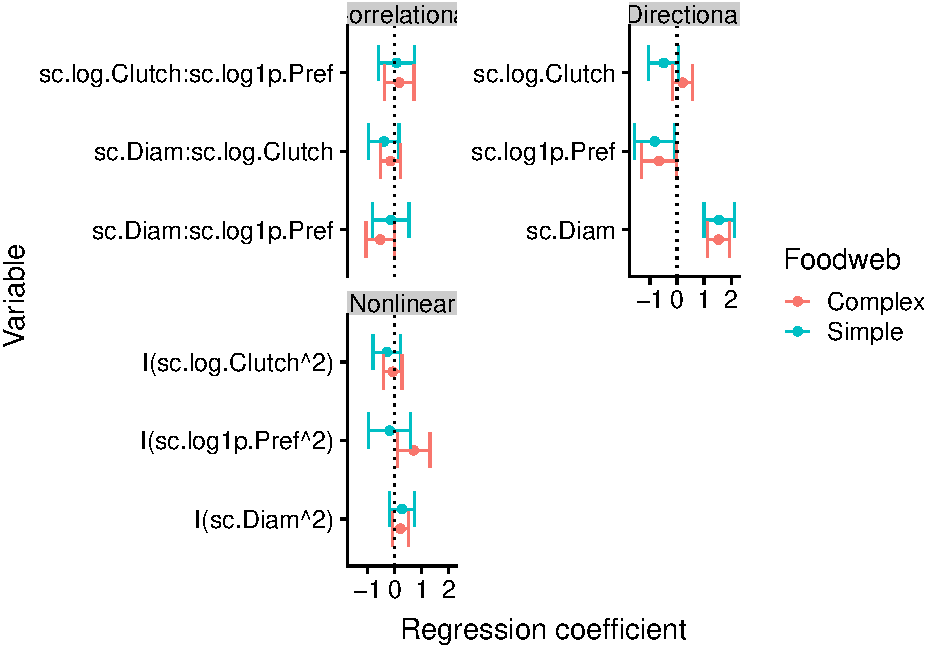
\includegraphics{ms_complexity_selection_files/figure-latex/Get Selection Gradients for GLMER-1.pdf}

\begin{Shaded}
\begin{Highlighting}[]
\NormalTok{## Modify to be directional, nonlinear, then correlational with legend in 4th area.}
\NormalTok{## Modify so that axes have gamma and beta with the trait as a subscript}
\KeywordTok{bind_rows}\NormalTok{(}\KeywordTok{mutate}\NormalTok{(}\KeywordTok{select}\NormalTok{(coefs_gradients, Variable, }\DataTypeTok{b=}\NormalTok{b_complex, }\DataTypeTok{b_2.5=}\NormalTok{b_complex_}\FloatTok{2.5}\NormalTok{, }\DataTypeTok{b_97.5=}\NormalTok{b_complex_}\FloatTok{97.5}\NormalTok{, Selection_form), }\DataTypeTok{Foodweb =} \StringTok{"Complex"}\NormalTok{),}
          \KeywordTok{mutate}\NormalTok{(}\KeywordTok{select}\NormalTok{(coefs_gradients, Variable, }\DataTypeTok{b=}\NormalTok{b_simple, }\DataTypeTok{b_2.5=}\NormalTok{b_simple_}\FloatTok{2.5}\NormalTok{, }\DataTypeTok{b_97.5=}\NormalTok{b_simple_}\FloatTok{97.5}\NormalTok{, Selection_form), }\DataTypeTok{Foodweb =} \StringTok{"Simple"}\NormalTok{)) }\OperatorTok
\StringTok{  }\KeywordTok{filter}\NormalTok{(Variable }\OperatorTok{!=}\StringTok{ "(Intercept)"}\NormalTok{) }\OperatorTok
\StringTok{  }\KeywordTok{ggplot}\NormalTok{(., }\KeywordTok{aes}\NormalTok{(}\DataTypeTok{x =}\NormalTok{ Variable, }\DataTypeTok{fill=}\NormalTok{Foodweb, }\DataTypeTok{color=}\NormalTok{Foodweb)) }\OperatorTok{+}
\StringTok{  }\KeywordTok{geom_point}\NormalTok{(}\KeywordTok{aes}\NormalTok{(}\DataTypeTok{y=}\NormalTok{b), }\DataTypeTok{position =} \KeywordTok{position_dodge}\NormalTok{(}\DataTypeTok{width=}\FloatTok{0.5}\NormalTok{)) }\OperatorTok{+}
\StringTok{  }\KeywordTok{geom_errorbar}\NormalTok{(}\KeywordTok{aes}\NormalTok{(}\DataTypeTok{ymax =}\NormalTok{ b_}\FloatTok{97.5}\NormalTok{, }\DataTypeTok{ymin =}\NormalTok{ b_}\FloatTok{2.5}\NormalTok{), }\DataTypeTok{position =} \KeywordTok{position_dodge}\NormalTok{(}\DataTypeTok{width=}\FloatTok{0.5}\NormalTok{)) }\OperatorTok{+}
\StringTok{  }\KeywordTok{coord_flip}\NormalTok{() }\OperatorTok{+}
\StringTok{  }\KeywordTok{geom_hline}\NormalTok{(}\DataTypeTok{yintercept=}\DecValTok{0}\NormalTok{, }\DataTypeTok{linetype=}\StringTok{"dotted"}\NormalTok{) }\OperatorTok{+}
\StringTok{  }\KeywordTok{facet_wrap}\NormalTok{(}\OperatorTok{~}\NormalTok{Selection_form, }\DataTypeTok{nrow=}\DecValTok{2}\NormalTok{, }\DataTypeTok{scales =} \StringTok{"free_y"}\NormalTok{) }\OperatorTok{+}
\StringTok{  }\KeywordTok{ylab}\NormalTok{(}\StringTok{"Selection gradient"}\NormalTok{)}
\end{Highlighting}
\end{Shaded}

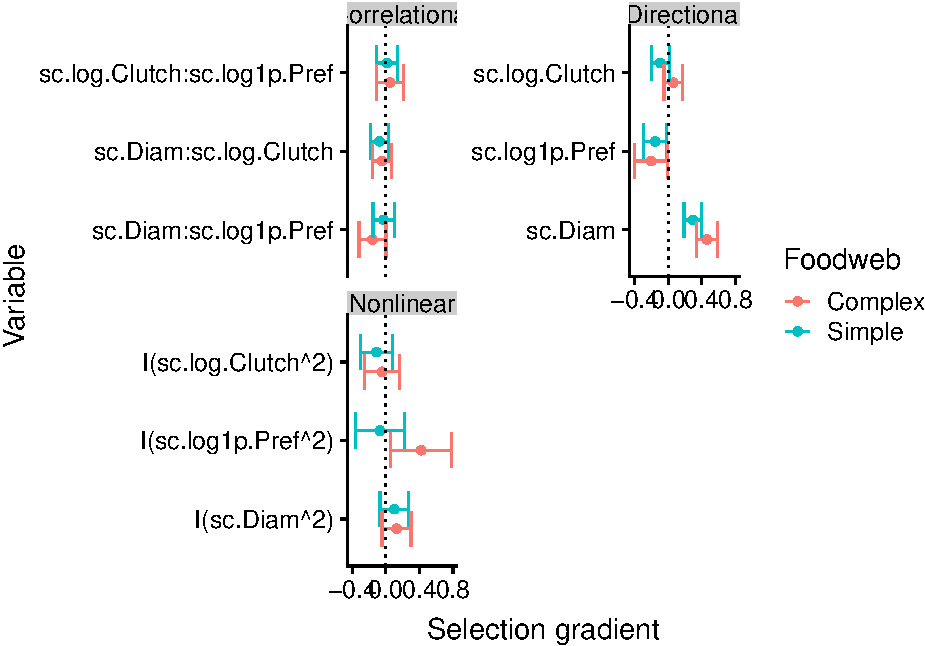
\includegraphics{ms_complexity_selection_files/figure-latex/Get Selection Gradients for GLMER-2.pdf}

What's the rationale for this test? First, we focus on galls where there
is evidence of both survival and parasitism within the gall. The idea is
that galls from the same clutch should be similar in size, therefore,
any selection on diameter would be apparent. If we assume that this is
all due to the effect of parasitism on larval development, truncating
gall diameter, then we can consider this new selection gradient to be
the result of confounding factors. Note that this is likely
overestimates the effect of the confounding factor, since we are
assuming that any heterogeneity in gall size (for this dataset) is due
to a confounding effect of parasitism on gall diameter. Then, we can
just subtract this value from the observed covariance between gall
diameter and larval survival to adjust for the confounding effects of
parasitism. This analysis should be relegated to the supplement.

Would we expect any confounding effects on nonlinear selection?

Appears to be selection for Platygaster to attack larva at high
densities in more complex food webs (and a decrease in the variance).
This may be a result of the poorer searching ability of parasitoids at
very high gall densities, potentially due to saturation. This suggests
that the fitness landscape may be dynamic because these selective
effects (assuming there is heritable variation in the egg parasitoid)
will change the following year. This could be an important discussion
point to take into account for future work. This is different from
simply altering the strength of selection, which will occur as species
move along the fitness landscape, but this result suggests that the
nature of the fitness landscape may actually be changing. For example,
larval parasitoids could be driving selection on Platygaster to be very
efficient at foraging, which will dampen once this pressure is removed,
and then could also dampen the selection acting on the galling
herbivore.

\subsection{Table for Alpha regression
coefficients}\label{table-for-alpha-regression-coefficients}

\begin{table}[]
\begin{tabular}{lcc}
                                                                           \\ \hline
                       & \multicolumn{2}{c}{Food web (Estimate [95\% CI])} \\
\textbf{Coefficient}   & \textbf{Complex} & \textbf{Simple}                \\ \hline
$Diam$                 & `r ` [`r `-`r `] & `r ` [`r `-`r `]  \\
$Clutch$               & `r ` [`r `-`r `] & `r ` [`r `-`r `]  \\
$Pref$                 & `r ` [`r `-`r `] & `r ` [`r `-`r `]  \\
$Diam^2$               & `r ` [`r `-`r `] & `r ` [`r `-`r `]  \\
$Clutch^2$             & `r ` [`r `-`r `] & `r ` [`r `-`r `]  \\
$Pref^2$               & `r ` [`r `-`r `] & `r ` [`r `-`r `]  \\
$Diam:Clutch$          & `r ` [`r `-`r `] & `r ` [`r `-`r `]  \\
$Diam:Pref$            & `r ` [`r `-`r `] & `r ` [`r `-`r `]  \\
$Clutch:Pref$          & `r ` [`r `-`r `] & `r ` [`r `-`r `]              \\ \hline
\end{tabular}
\end{table}

\subsection{Table for Iteomyia selection
gradients}\label{table-for-iteomyia-selection-gradients}

\begin{table}[]
\begin{tabular}{lcc}
                                                                                  \\ \hline
                                  & \multicolumn{2}{c}{Food web (Estimate [95\% CI])} \\
\textbf{Selection gradient}       & \textbf{Complex} & \textbf{Simple}            \\ \hline
$\beta_{Diam}$                    & `r ` [`r `-`r `] & `r ` [`r `-`r `]  \\
$\beta_{Clutch}$                  & `r ` [`r `-`r `] & `r ` [`r `-`r `]  \\
$\beta_{Pref}$                    & `r ` [`r `-`r `] & `r ` [`r `-`r `]  \\
$\gamma_{Diam,Diam}$              & `r ` [`r `-`r `] & `r ` [`r `-`r `]  \\
$\gamma_{Clutch,Clutch}$          & `r ` [`r `-`r `] & `r ` [`r `-`r `]  \\
$\gamma_{Pref,Pref}$              & `r ` [`r `-`r `] & `r ` [`r `-`r `]  \\
$\gamma_{Diam,Clutch}$            & `r ` [`r `-`r `] & `r ` [`r `-`r `]  \\
$\gamma_{Diam,Pref}$              & `r ` [`r `-`r `] & `r ` [`r `-`r `]  \\
$\gamma_{Clutch,Pref}$            & `r ` [`r `-`r `] & `r ` [`r `-`r `]           \\ \hline
\end{tabular}
\end{table}

\subsection{Table for bias}\label{table-for-bias}

\begin{table}[]
\begin{tabular}{lc}
                                                                  \\ \hline
\textbf{Type}                 & \textbf{Bias} \boldmath$s_{Diam}$ \\ \hline
Complex (All)                 & `r ` [`r `-`r `]  \\
Complex (Larval guild)        & `r ` [`r `-`r `]  \\
Simple (\textit{Platygaster}) & `r ` [`r `-`r `]                  \\ \hline
\end{tabular}
\end{table}

\subsection{Table for Platygaster
selection}\label{table-for-platygaster-selection}

\begin{table}[]
\begin{tabular}{lc}
                                                                  \\ \hline
\textbf{Selection differential} & \textbf{Estimate [95\% CI]}     \\ \hline
$s_{Diam}$                      & `r ` [`r `-`r `]  \\
$s_{Clutch}$                    & `r ` [`r `-`r `]  \\
$s_{Pref}$                      & `r ` [`r `-`r `]  \\ 
$s_{Diam,Diam}$                 & `r ` [`r `-`r `]  \\
$s_{Clutch,Clutch}$             & `r ` [`r `-`r `]  \\
$s_{Pref,Pref}$                 & `r ` [`r `-`r `]                \\ \hline
\end{tabular}
\end{table}

Note that equation 3 in Phillips and Arnold 1998 is good justification
for why quadratic selection cofficients should be multiplied by two (but
not correlational ones?)

The G-matrix is essentially a scalar. For my data, since there is no
correlational selection, it doesn't matter if there is genetic
covariance between the traits, as this will not effect the change in
genetic covariances within a generation (because there is no selection).
Also, the G\_matrix does not qualitatively alter the conclusions that
there will be a decrease in additive genetic variance in gall diameter
due to the strong directional selection; however, there will be an
increase in the additive genetic variance in female preference. Since
this is an experiment, we can assume that the G-matrix is the same
between treatments

Remember that the diagonals refer to additive genetic CO-variances.
Thus, positive or negative values for delta\_G give insight to whether
selection will act to integrate traits (positive covariance) or create
trade-offs (negative covariance).

Assuming that there is positive additive genetic variance and
co-variance in these traits (i.e.~all values of G-matrix are positive),
then the curvature of the fitness landscape can give insight to
qualitative changes in the G matrix. This is because the G-matrix acts
as a scalar of changes in the fitness landscape.

Compared to the GLM, the GLMM gives the same inferences about the effect
of food-web treatment. The main difference was that there was stronger
evidence of correlational selection, but no evidence that this
correlational selection varied among food-web treatments. Still, this
stronger evidence for correlational selection should be interpreted with
caution since the GLM does not account for the non-indepedence of these
fitness estimates.

\section{Results}\label{results}

We found that changes in food-web complexity altered the shape of
\emph{Iteomyia}'s fitness landscape ().

For example, there was directional selection for larger gall diameter in
both complex and simple food webs, but the magnitude of the selection
gradient was X-fold higher in the complex food web. The steeper
selection gradient in the complex food web was not a result of stronger
covariance between gall diameter and larval survival, but a result of
average larval survival being X-fold lower in the complex food web.

We observed directional selection for smaller clutch sizes in the simple
food web, but no evidence of selection on this trait in the complex food
web. The absence of selection in the complex food web appeared to be a
result of conflicting selection pressures imposed by the egg parasitoid
\emph{Platygaster} and the guild of larval parasitoids (statistical test
focus on egg vs.~larval parasitoids). Specifically, larval parasitoids
actually impose directional selection for larger clutch sizes (selection
gradient), but the net effect is no selection when both parasitoid
guilds are present.

We found evidence of disruptive selection acting on female preference in
the complex food web, but no evidence of nonlinear selection on this
trait in the simple food web. Similar to clutch size, these differences
in nonlinear selection appeared to be due to different selection
pressures imposed by egg and larval parasitoids.

\textbf{Characterizing the slope and curvature of the fitness landscape}

\textbf{Old}

\section{Discussion}\label{discussion}

Our key finding was that the adaptive landscape was less constrained in
the complex vs.~simple food web. These fewer constraints arise from
conflicting selection pressures imposed by different parasitoid guilds,
resulting in fewer traits under selection in the complex food web. At
the same time, we observed an overall greater intensity of selection in
the complex food web, suggesting that trait evolution can be faster in
complex vs.~simple food webs. Our observation that natural selection was
more constrained and less intense in simple vs.~complex food webs
suggests that the loss of biodiversity could constrain the adaptive
potential of interacting species by reducing genetic and phenotypic
variation in multiple traits.

Current theory suggests that when the number of selective constrains is
less than the number of genetic constraints (i.e.~some genetically
variable traits are selective neutral), there are multiple positions on
the landscape that confer equal fitness (Lande 1981; Lande and Arnold
1985). In this scenario, trait differences between populations may
simply be due to neutral processes (e.g.~genetic drift and mutation)
moving trait values of the population. For our system, we currently lack
quantitative estimates of genetic variation in our traits, although work
with other species of galling insects has shown that gall diameter
(Abramhson, Heath's work), clutch size (look to Weiss' work), and
oviposition preference (Abrahmson's work?) are genetically variable. We
encourage others to examine how changes in community context will alter
selection on multiple traits.

One interesting result of our work was that the overall intensity of
selection appeared to be larger in complex food webs. This result was
driven by the large selection gradient acting on gall diameter in
complex vs.~simple food webs. This difference in selection intensity is
likely not driven by a difference in the ecological relationship between
gall diameter and parasitoid attack (i.e.~slope), but actually a result
of the lower mean fitness of \emph{Iteomyia} in the complex food web.
This lower mean fitness is not surprising ---we excluded an entire guild
of parasitoids from attacking the insect. But this more intense
selection pressure may simply represent a transient dynamic. This is
because we would expect the egg-parasitoid \emph{Platygaster} to
increase in abundance over time once its intraguild predator has been
removed. While our results suggest that this wouldn't affect the slope
of the relationship, the higher abundance of the egg parasitoid would
likely reduce the mean fitness of \emph{Iteomyia}, thus increasing the
selection gradient acting on gall diameter closer to what we observed in
the complex food web. We don't expect it to fully compensate, given that
the larval parasitoids exhibit a different functional relationship with
gall traits, and thus we expect a more diverse community of primary
parasitoids to generally impose greater parasitism pressure, a factor
that appears to be a general trend in parasitoid community (Hawkins
citation) and likely for other consumers (Ives and Cardinale Ecology
Letters).

Our study focused on quantifying the direct effects of changes in
network complexity on the fitness landscape; however, changes in network
complexity may have pervasive indirect effects via coevolution or by
initiating evolutionary cascades. In our system, we observed that
excluding the guild of larval parasitoids altered selection on both the
basal resource (\emph{Iteomyia}) and the intraguild prey
(\emph{Platygaster}). GIVE DETAILS AND SUGGEST A POTENTIAL EVOLUTIONARY
CASCADE.

Our study manipulated food-web complexity and examined changes in the
fitness landscape of species embedded within this network. However,
other studies have also examined, at least theoretically, how changes in
the diversity of competitive communities affects evolution. These
studies have generally suggested that the diversity of competitors may
actually constrain the adaptive landscape, a finding that stands in
contrast to our results. NEED TO REVIEW THESE PAPERS TO SEE HOW ITS
DIFFERENT.

We suggest that by explicitly focusing on network structure, we can
predict how changes in biodiversity will affect the adaptive potential
of constituent species. A network allows a powerful representation of
the `community context', lending predictive power to how changes in
network structure (either due to loss of species or links), will alter
natural selection and consequently evolutionary change. Our results also
suggest that losing biodiversity may not just have consequences at the
community level, but also population-level consequences that may
actually constrain adaptation to changing environments. This argues that
changes in network complexity may not only affect the robustness of
communities, but also that of constituent populations to future
environmental change.

\section*{References}\label{references}
\addcontentsline{toc}{section}{References}

\hypertarget{refs}{}
\hypertarget{ref-Barbour2016}{}
Barbour, Matthew A, Miguel A Fortuna, Jordi Bascompte, Joshua R
Nicholson, Riitta Julkunen-Tiitto, Erik S Jules, and Gregory M
Crutsinger. 2016. ``Genetic Specificity of a Plant--insect Food Web:
Implications for Linking Genetic Variation to Network Complexity.''
\emph{Proceedings of the National Academy of Sciences} 113 (8). National
Acad Sciences: 2128--33.

\hypertarget{ref-Barbour2015}{}
Barbour, Matthew A, Mariano A Rodriguez-Cabal, Elizabeth T Wu, Riitta
Julkunen-Tiitto, Carol E Ritland, Allyson E Miscampbell, Erik S Jules,
and Gregory M Crutsinger. 2015. ``Multiple Plant Traits Shape the
Genetic Basis of Herbivore Community Assembly.'' \emph{Funct. Ecol.} 29
(8): 995--1006.

\hypertarget{ref-Bolker2009}{}
Bolker, Benjamin M, Mollie E Brooks, Connie J Clark, Shane W Geange,
John R Poulsen, M Henry H Stevens, and Jada-Simone S White. 2009.
``Generalized Linear Mixed Models: A Practical Guide for Ecology and
Evolution.'' \emph{Trends Ecol. Evol.} 24 (3): 127--35.

\hypertarget{ref-Janzen1998}{}
Frederic J Janzen and Hal S Stearn. 1998. ``Logistic Regression for
Empirical Studies of Multivariate Selection.'' \emph{Evolution} 52 (6):
1564--71.

\hypertarget{ref-Gripenberg2010}{}
Gripenberg, Sofia, Peter J Mayhew, Mark Parnell, and Tomas Roslin. 2010.
``A Meta-Analysis of Preference-Performance Relationships in
Phytophagous Insects.'' \emph{Ecol. Lett.} 13 (3): 383--93.

\hypertarget{ref-Hawkins1997}{}
Hawkins, Bradford A, Howard V Cornell, and Michael E Hochberg. 1997.
``Predators, Parasitoids, and Pathogens as Mortality Agents in
Phytophagous Insect Populations.'' \emph{Ecology} 78 (7). Ecological
Society of America: 2145--52.

\hypertarget{ref-Heath2018}{}
Heath, Jeremy J, Patrick Abbot, and John O Stireman 3rd. 2018.
``Adaptive Divergence in a Defense Symbiosis Driven from the Top down.''
\emph{Am. Nat.} 192 (1): E21--E36.

\hypertarget{ref-Hunter2018}{}
Hunter, Darren C, Josephine M Pemberton, Jill G Pilkington, and Michael
B Morrissey. 2018. ``Quantification and Decomposition of
Environment-Selection Relationships.'' \emph{Evolution}, March.

\hypertarget{ref-Ives2005}{}
Ives, Anthony R, Bradley J Cardinale, and William E Snyder. 2005. ``A
Synthesis of Subdisciplines: Predator--prey Interactions, and
Biodiversity and Ecosystem Functioning.'' \emph{Ecol. Lett.} 8 (1).
Blackwell Science Ltd: 102--16.

\hypertarget{ref-R2018}{}
R Core Team. 2018. \emph{R: A Language and Environment for Statistical
Computing}. Vienna, Austria: R Foundation for Statistical Computing.
\url{https://www.R-project.org/}.

\hypertarget{ref-Russo2006}{}
Russo, Ron. 2006. \emph{Field Guide to Plant Galls of California and
Other Western States}. 1st ed. University of California Press.

\hypertarget{ref-Singer1986}{}
Singer, Michael C. 1986. ``The Definition and Measurement of Oviposition
Preference in Plant-Feeding Insects.'' In \emph{Insect-Plant
Interactions}, edited by James R Miller and Thomas A Miller, 65--94. New
York, NY: Springer New York.

\hypertarget{ref-Weis1983}{}
Weis, Arthur E, Peter W Price, and Michael Lynch. 1983. ``Selective
Pressures on Clutch Size in the Gall Maker Asteromyia Carbonifera.''
\emph{Ecology} 64 (4). Ecological Society of America: 688--95.

\end{document}


